% Body of the 6-page FIST-2027 version. Included by fist_blind.tex and fist_named.tex (\ifblind switches the author block and the availability sentence).
% Tables come from ../tables (generated by experiments/paper_tables.py); every number is audited by paper/check_text_numbers.py.
\usepackage{amsmath,amssymb,amsfonts}
\usepackage{fontspec}  % Tectonic is XeTeX-based: load a Times-compatible text font (IEEE conference papers are set in Times); math stays Computer Modern
\setmainfont{texgyretermes-regular.otf}[BoldFont=texgyretermes-bold.otf, ItalicFont=texgyretermes-italic.otf, BoldItalicFont=texgyretermes-bolditalic.otf]
\setsansfont{texgyreheros-regular.otf}[BoldFont=texgyreheros-bold.otf, ItalicFont=texgyreheros-italic.otf, BoldItalicFont=texgyreheros-bolditalic.otf]
\setmonofont{texgyrecursor-regular.otf}[BoldFont=texgyrecursor-bold.otf, ItalicFont=texgyrecursor-italic.otf, BoldItalicFont=texgyrecursor-bolditalic.otf]
\usepackage{graphicx}
\usepackage{booktabs}
\usepackage{array}
\usepackage{xcolor}
\usepackage{algorithm}
\usepackage{algpseudocode}
\usepackage{tikz}
\usetikzlibrary{arrows.meta,positioning}
\usepackage{cite}
\usepackage[hyphens]{url}
\Urlmuskip=0mu plus 1mu

\newcommand{\qbar}{\ensuremath{\bar q}}
\newcommand{\phat}{\ensuremath{\hat p}}
\newcommand{\shat}{\ensuremath{\hat\sigma}}
\newcommand{\Stilde}{\ensuremath{\tilde S}}
\newcommand{\Atrain}{\ensuremath{A_{\mathrm{train}}}}
\newcommand{\Atest}{\ensuremath{A_{\mathrm{test}}}}

\begin{document}

\title{Beyond $k$-Anonymity in Password Breach Checking:\\ How Robust Is Frequency-Smoothing Bucketization?}
\ifblind
\author{\IEEEauthorblockN{Anonymous Authors}\IEEEauthorblockA{Affiliation withheld for double-blind review}}
\else
\author{\IEEEauthorblockN{Dilpreet Singh, Ishita Gupta and Madhav Raj}\IEEEauthorblockA{National Institute of Technology Delhi, India}\and\IEEEauthorblockN{Dr.\ Sandhya Pundhir}\IEEEauthorblockA{Dept.\ of Computer Science and Engineering\\National Institute of Technology Delhi, India}}
\fi
\maketitle

\begin{abstract}
Frequency-smoothing bucketization (FSB) lets a compromised-credential-checking server hide which leaked password a client asks about, but its guarantee holds only relative to the server's own estimate of the password distribution. We measure by simulation on the RockYou leak (13.1M stored passwords, held-out accounts as targets) how far that guarantee carries when the estimate is noisy and the attacker holds the leak. Against the estimate-based attacker of Li et al., FSB's loss over the no-bucket baseline is 0.0 percentage points (pp) at $q=\qbar=100$ guesses, against 41.1 pp for size-matched hash-prefix bucketization (HPB), and it tolerates multiplicative noise of about $\sigma=0.7$ on the estimate. A count-aware attacker is stronger: FSB then loses 10.5 to 10.9 pp at $q=\qbar$, still about 73\% below HPB. The loss comes from rare stored passwords that the estimate underrates. A floor on the number of buckets per password removes most of it for $q\le\qbar$ (0.08 pp at $\qbar=100$ for 1.56 times the bucket size) but not beyond $\qbar$, and the results are stable over four splits of the leak.
\end{abstract}

\begin{IEEEkeywords}
compromised credential checking, password breach, frequency-smoothing bucketization, $k$-anonymity, privacy, password guessing
\end{IEEEkeywords}

\section{Introduction}

Compromised-credential checking (C3) services let a client find out whether a password appears in a breach corpus without sending it in the clear. Have I Been Pwned (HIBP)~\cite{hunt} and Google Password Checkup~\cite{thomas2019} divide the leaked data into buckets, and the client reveals only the identifier of the bucket its credential would fall in, before a private-set-intersection step inside that bucket. Li et al.~\cite{li2019} showed that a revealed hash prefix is not harmless: a server that sees it can guess the password with far better odds than one that does not.

They proposed frequency-smoothing bucketization (FSB), which uses an estimate of the password distribution to store popular passwords in several buckets, so that the revealed bucket is close to uniform given the password. Against an attacker who knows the same estimate, FSB leaks almost nothing at the guess budgets they study. The guarantee is therefore relative to the estimate, and two questions decide whether FSB is safe to deploy. \emph{How wrong can the estimate be?} It is built from a leak and a language model and is never exact. \emph{How strong can the attacker be?} Li et al.\ note that their simulated attacker ranks guesses with the server's estimate and is not optimal; an attacker that ranks by the leak counts has not, to our knowledge, been measured.

We answer both with a measurement study on a 14M-password RockYou corpus. The server stores $N=13{,}125{,}513$ distinct passwords in $2^{24}$ buckets, with an estimate made of a histogram head of the top $t=1{,}000{,}000$ passwords and a character 3-gram tail. We compare FSB with size-matched HPB, giving HPB the larger bucket whenever the two cannot match exactly (up to 25\% larger), so any advantage we report for FSB is conservative. Our contributions are five measurements.
\begin{enumerate}
\item \textbf{Reproduction and noise tolerance.} Against the estimate-based attacker FSB's loss at $q=\qbar$ is 0.0 pp for $\qbar=10$, 100 and 1000, while size-matched HPB loses 37.0, 41.1 and 40.2 pp. The loss reaches 5 pp at noise $\sigma=0.87$, 0.69 and 0.66, against a measured head error $\shat=0.31$ (a margin of about two to one).
\item \textbf{A count-aware attacker.} An attacker that ranks by leak counts gains 10.5, 10.9 and 10.9 pp at $q=\qbar$, still about 73\% less than HPB; under a policy that rejects short and blocklisted passwords FSB removes less than 1\% of HPB's loss at $q=1$ for $\qbar=100$.
\item \textbf{Mechanism.} The residual loss is on rare passwords stored outside the histogram head (leak count 1 or 2 for 98.6\% of the targets gained at $q=1$), while HPB leaks the popular head passwords.
\item \textbf{A floor on $\gamma$.} Storing every string in at least $g$ buckets tests the mechanism by intervention: for $\qbar=100$ and $g=2{,}048$ the worst-case loss over three attackers at $q=\qbar$ falls from 10.68 to 0.08 pp on a fresh pool at 1.56 times the average bucket. It does not help for $q>\qbar$.
\item \textbf{Stability.} Over four independent splits of the leak the worst-case loss at $q=\qbar=100$ on M0 is $10.96\pm0.06$ pp for plain FSB and $0.10\pm0.03$ pp with the floor.
\end{enumerate}

\section{Background}

A C3 server holds a set $S$ of leaked passwords and publishes a bucketization: each stored password is assigned to one or more of $|B|$ buckets. To check a password $w$ the client picks a bucket that contains $w$, sends its identifier, and the two parties run a private-set-intersection protocol on that bucket; the server learns the identifier and nothing else, so the choice of bucket is the leakage we study. We treat the server as honest-but-curious, as Li et al.~\cite{li2019} do, and the protocol inside the bucket as ideal.

\textbf{HPB.} HIBP-style services assign $w$ to the bucket named by the first $l$ bits of its hash, so each password lives in exactly one bucket of about $|S|/2^l$ entries; a bucket concentrates the probability mass of every popular password it contains.

\textbf{FSB.} Given an estimate $\phat$ of the password distribution and a guess budget $\qbar$, let $w_{\bar q}$ be the $\qbar$-th most probable password under $\phat$. Password $w$ is stored in $\gamma(w)$ buckets and the client picks one of them uniformly at random:
\begin{equation}\label{eq:gamma}
\gamma(w) = \min\left(|B|,\ \left\lceil |B| \cdot \frac{\hat p(w)}{\hat p(w_{\bar q})} \right\rceil\right).
\end{equation}
The $\gamma(w)$ buckets are consecutive identifiers (modulo $|B|$) starting at $f(w)$, the first $\log_2|B|$ bits of the salted SHA-256 of $w$ (Algorithm~\ref{alg:fsb}). The most popular passwords therefore sit in many buckets and rare ones in few. Li et al.\ show that if the attacker ranks with the same $\phat$ and $\phat$ equals the true distribution, seeing the bucket gains nothing as long as $q\le\qbar$; the price is bandwidth. A floor $g$ on the number of copies replaces $\gamma$ by
\begin{equation}\label{eq:floor}
\gamma_g(w)=\min\bigl(|B|,\ \max(\gamma(w),\,g)\bigr),
\end{equation}
and $g=1$ is plain FSB.

\begin{algorithm}[t]
\caption{FSB with a floor $g$ ($g=1$: plain FSB); $b=\log_2|B|$.}
\label{alg:fsb}
\begin{algorithmic}[1]
\Function{Buckets}{$w$}
  \State $\gamma \gets \min\bigl(|B|,\ \max(g,\ \lceil |B|\,\hat p(w)/\hat p(w_{\bar q})\rceil)\bigr)$
  \State $f \gets$ the first $b$ bits of $h(w)$
  \State \Return $\{(f+i) \bmod |B| : i=0,\dots,\gamma-1\}$
\EndFunction
\Function{ClientQuery}{$w$}
  \State draw $j$ uniformly from \Call{Buckets}{$w$}; send $j$
\EndFunction
\Function{ServerBucket}{$j$}
  \State \Return $\{w\in\tilde S : (j-f(w)) \bmod |B| < \gamma(w)\}$
\EndFunction
\end{algorithmic}
\end{algorithm}

\textbf{The estimate.} Following Li et al., $\phat$ stores the top $t=1{,}000{,}000$ passwords of the training leak by count (the head $H_t$) and scores every other string with a character 3-gram model with add-$\delta$ smoothing ($\delta=0.01$), rescaled so the tail mass is consistent with the head:
\begin{equation}\label{eq:est}
\hat p(w)=\begin{cases} p_h(w) & w\in H_t,\\[2pt] p_n(w)\,\dfrac{1-\sum_{v\in H_t}p_h(v)}{1-\sum_{v\in H_t}p_n(v)} & \text{otherwise,}\end{cases}
\end{equation}
where $p_h$ is the histogram probability (count over total) and $p_n$ the 3-gram probability.

\section{Threat Model and Experimental Setup}

\textbf{Threat model.} A C3 server, or anyone who reads its logs, sees the bucket identifier $j$ of a client's query and tries to guess the client's password within $q$ guesses (Fig.~\ref{fig:system}). The attacker knows the bucketization, including $\phat$ and the bucket contents, and has no other side information: we model password-only checking, as in HIBP and FSB. The property at stake is the \emph{privacy} of the queried password against the server; FSB does not improve the security of any account and says nothing about integrity or availability. A malicious client, an actively malicious server and repeated queries of one password are outside our measurements.

\begin{figure}[t]
\centering
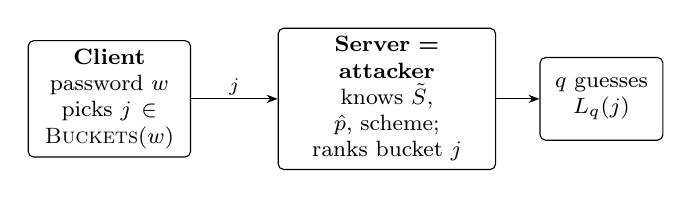
\begin{tikzpicture}[font=\footnotesize, box/.style={draw, rounded corners=2pt, align=center, inner sep=3pt, minimum height=1.05cm}, >={Stealth[length=4pt]}]
\node[box, text width=1.85cm] (c) {\textbf{Client}\\ password $w$\\ picks $j\in\textsc{Buckets}(w)$};
\node[box, text width=2.55cm, right=1.1cm of c] (s) {\textbf{Server = attacker}\\ knows $\tilde S$, $\hat p$, scheme;\\ ranks bucket $j$};
\node[box, text width=1.35cm, right=0.55cm of s] (g) {$q$ guesses\\ $L_q(j)$};
\draw[->] (c) -- node[above, font=\scriptsize, inner sep=1pt]{$j$} (s);
\draw[->] (s) -- (g);
\end{tikzpicture}
\caption{System and threat model: the honest-but-curious server sees only the bucket identifier $j$, knows $\tilde S$, $\hat p$ and the scheme, and wins if the client's password is among its $q$ guesses.}
\label{fig:system}
\end{figure}

\textbf{Data.} The leak is RockYou (14,326,970 unique passwords, 32,581,870 accounts after cleaning to printable ASCII of length 1 to 30), the largest public leak of real, user-chosen passwords with occurrence counts that we found in SecLists~\cite{miessler}. It is dominated by rare passwords (82.8\% of its unique passwords occur once, while the top 1,000 cover 11.30\% of accounts), the regime in which an estimate of the tail matters; it is a 2009 leak from one site, so we do not claim that its tail matches other populations. We split its accounts at random: 90\% form the training leak \Atrain, which the server stores as $\Stilde$ ($N=13{,}125{,}513$) and uses to build $\phat$, and the other 10\% form the target pool \Atest. phpbb (184,381 unique passwords, 88.6\% singletons) is a small out-of-distribution target pool. The server has $2^{24}$ buckets.

\textbf{Attackers.} Both attackers see the bucket $j$ and rank the stored candidates $c$ with $j\in\textsc{Buckets}(c)$ by
\begin{equation}\label{eq:score}
s(c)=a(c)\,/\,\gamma(c),
\end{equation}
breaking ties by $a(c)$ and then lexicographically, and guess the top $q$. They differ in the weight $a(c)$. \textbf{est} uses $a(c)=\phat(c)$, the information Li et al.\ give the attacker (the 2M most probable passwords; using all of $\Stilde$ changes nothing for $q\le\qbar$). \textbf{emp} uses the leak count of $c$, as an attacker holding the same leak would, over all 13.1M stored passwords; it generates no strings absent from the leak, so its results are lower bounds, and it is our headline attacker. A third attacker, \textbf{gt}, is introduced with the floor (Section~\ref{sec:floor}).

\textbf{Metric.} For each target we play the client's side and let the attacker guess. The baseline is the same attacker's success without a bucket (its top $q$ candidates overall), and the loss, in percentage points (pp), is
\begin{equation}\label{eq:loss}
\mathrm{loss}(q)=\mathrm{success}_{\text{bucket}}(q)-\mathrm{success}_{\text{baseline}}(q).
\end{equation}
We use 5 repeats of 5,000 targets drawn in proportion to leak count and report the standard deviation over repeats. Targets outside $\Stilde$ can never be guessed, so they add nothing to the loss.

\textbf{Size matching and conditions.} FSB with $\qbar=10$, 100 and 1000 has an average bucket of 790, 2,565 and 11,336 entries; HPB at the nearest power-of-two prefix length ($l=14$, 12, 10) has 801, 3,204 and 12,818, i.e.\ 1\%, 25\% and 13\% larger, which favours HPB. Conditions: M0, targets from \Atest; M1b, phpbb targets; M2x, \Atest\ targets with length $\ge 8$ and not on the Xato top-370 list~\cite{miessler}, with attacker candidates restricted likewise but the server's estimate unchanged (a site that forbids weak passwords); M3, $\phat$ multiplied by $\exp(\sigma z_w)$ with $z_w$ a fixed per-password standard normal.

\textbf{Implementation.} The simulator is Python with NumPy and Numba (Python 3.12, NumPy 2.5.4, Numba 0.68.1, pandas 3.1.1 and SciPy 1.18.1, on a laptop with an Apple M5 processor (10 cores, 16 GB RAM)). Bucket sizes are counted exactly with a difference array over the circular ranges, and a bucket query is answered by binary search over start-sorted classes of equal $\gamma$, never by a scan of $\tilde S$. All random choices are seeded (split seeds 101, 102 and 103; targets with seed 2000, 5000 and 6000 for the test, development and fresh pools), every result row carries a configuration hash, and one command regenerates every table and number.

\section{Results}

Unless stated otherwise $t=1{,}000{,}000$, the pool is \Atest, losses are in pp at $q=\qbar$, and $\pm$ is the standard deviation over 5 repeats.

\subsection{FSB holds against the estimate-based attacker}

With est, FSB loses 0.00 pp for every $q\le\qbar$ and every $\qbar\in\{10,100,1000\}$ on M0 and on M1b, while size-matched HPB loses 37.0, 41.1 and 40.2 pp at $q=\qbar$ on M0 (Table~\ref{tab:headline}) and 31.5, 35.7 and 36.1 pp on M1b. This reproduces the qualitative result of Li et al.\ on a smaller leak. The guarantee stops at $\qbar$ (Fig.~\ref{fig:loss}): at $q=1000$ with $\qbar=100$ the FSB loss is above 10 pp. Under the policy (M2x) the est loss is no longer zero, 0.96, 2.10 and 3.89 pp, as in the policy experiment of Li et al.

\begin{figure*}[t]
\centering
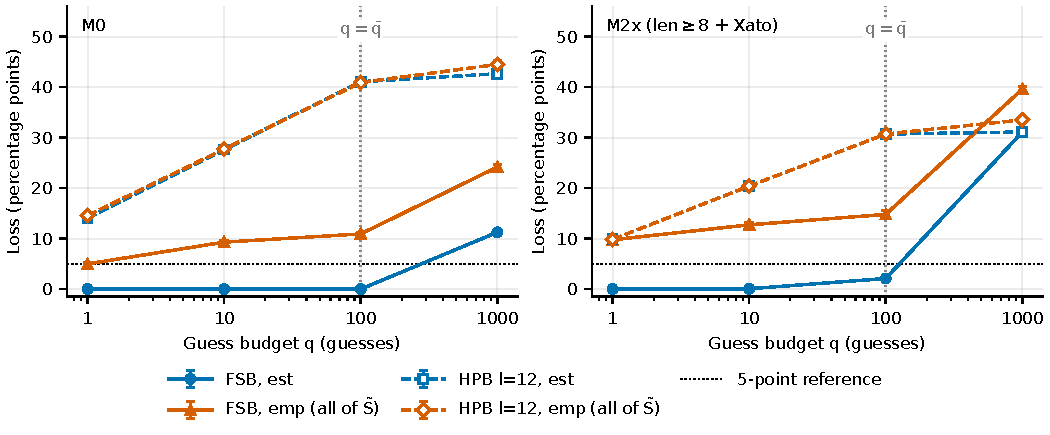
\includegraphics[width=\textwidth]{../figs/fig1_wide.pdf}
\caption{Loss against guess budget $q$ (log scale) for M0 (a) and M2x (b): FSB with $\qbar=100$ and size-matched HPB with $l=12$ (average bucket 2,565 and 3,204 entries), against the est and emp attackers. Dotted vertical line: $q=\qbar$; dotted horizontal line: 5 pp. At $q=\qbar=100$ on M0: FSB est 0.00, FSB emp 10.92, HPB emp 40.90 pp; on M2x: FSB est 2.10, FSB emp 14.79, HPB emp 30.70 pp. Error bars: sd over 5 repeats of 5,000 targets.}
\label{fig:loss}
\end{figure*}

With M3 the loss at $q=\qbar$ reaches 5 pp at $\sigma=0.874\pm0.059$, $0.693\pm0.027$ and $0.658\pm0.013$ for $\qbar=10$, 100 and 1000 (mean and sd over 5 noise draws). On held-out data the head of our estimate has a per-password dispersion $\shat=0.31$ (standard error 0.01; 0.11 when binned by mass, a lower bound), so the margin is about two to one. The tail is far worse ($\shat=1.57$, bias $+5.86$ log units: stored tail passwords are underestimated by a factor of about 350), but noise on tail strings alone moves the est loss by less than 1 pp up to $\sigma=1.6$ (Fig.~\ref{fig:noise}).

\begin{figure}[t]
\centering
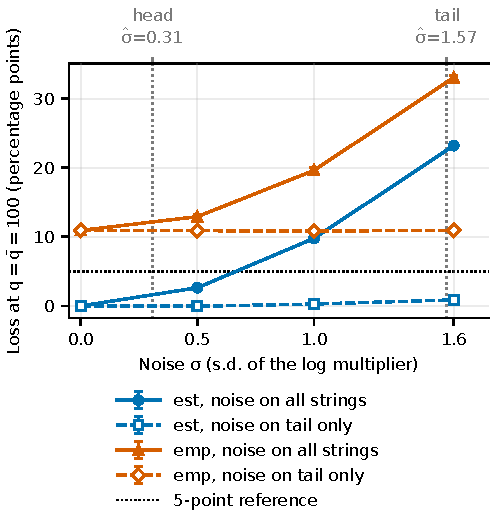
\includegraphics[width=\columnwidth]{../figs/fig2.pdf}
\caption{Loss at $q=\qbar=100$ (M0, FSB) against the noise $\sigma$ on $\phat$, for noise on every string and on tail strings only, est and emp (mean over 5 draws, bars: sd). Vertical lines: measured $\shat$, head 0.308 and tail 1.570; horizontal line: 5 pp. Tail-only noise leaves emp at the clean 10.92 pp (10.88, 10.84 and 10.94 at $\sigma=0.5$, 1.0 and 1.6); noise on every string raises it to 12.92, 19.60 and 33.03.}
\label{fig:noise}
\end{figure}

\begin{table*}[t]
\centering
\caption{Loss at $q=\bar q$ in pp (mean $\pm$ sd over 5 repeats). ``Removed'' is the share of the size-matched HPB loss that FSB removes (emp).}
\label{tab:headline}
\footnotesize
\begin{tabular}{llrrrrr}
\toprule
Cond. & $\bar q$ & Avg.\ bucket & \multicolumn{3}{c}{Loss at $q=\bar q$ (pp)} & Removed \\
\cmidrule(lr){4-6}
 & & (entries) & FSB est & FSB emp & HPB emp & (\%) \\
\midrule
M0 & 10 & 790 & $0.00 \pm 0.00$ & $10.52 \pm 0.39$ & $37.09 \pm 0.56$ & $72$ \\
 & 100 & 2,565 & $0.00 \pm 0.00$ & $10.92 \pm 0.35$ & $40.90 \pm 0.65$ & $73$ \\
 & 1000 & 11,336 & $0.00 \pm 0.00$ & $10.91 \pm 0.35$ & $39.69 \pm 0.89$ & $73$ \\
\midrule
M2x & 10 & 790 & $0.96 \pm 0.09$ & $13.54 \pm 0.43$ & $27.82 \pm 0.35$ & $51$ \\
 & 100 & 2,565 & $2.10 \pm 0.24$ & $14.79 \pm 0.69$ & $30.70 \pm 0.40$ & $52$ \\
 & 1000 & 11,336 & $3.89 \pm 0.23$ & $16.59 \pm 0.35$ & $29.84 \pm 0.27$ & $44$ \\
\bottomrule
\end{tabular}

\end{table*}

\subsection{An attacker who holds the leak}

emp gains $10.52\pm0.39$, $10.92\pm0.35$ and $10.91\pm0.35$ pp against FSB at $q=\qbar$ for $\qbar=10$, 100 and 1000 on M0 (Table~\ref{tab:headline}), against 37.1, 40.9 and 39.7 pp against size-matched HPB, so FSB still removes 72 to 73\% of the loss (77 to 78\% on M1b). At $q=1$ FSB's loss is 5.82, 4.99 and 3.97 pp against 21.10, 14.55 and 8.91 pp for HPB.

A password policy erases the benefit at $q=1$. Under M2x the popular passwords are gone and the baseline success at $q=1$ falls from 0.97\% to 0.12\%; the losses for $\qbar=100$ are then 9.76 pp for FSB and 9.84 pp for HPB, so FSB removes under 1\% of HPB's loss. At $\qbar=1000$ and $q=1$ FSB leaks more than HPB (8.58 against 6.06 pp, i.e.\ it removes $-41.7$\% of HPB's loss), even though HPB's buckets are 13\% larger.

\subsection{Where the loss comes from}

We split the targets into the head (the top $t$ passwords by count; 50.8\% of the M0 targets), the stored tail (in $\Stilde$ but outside the head; 11.7\%) and targets not in $\Stilde$ (37.5\%, never guessable). The loss splits as share $\times$ (success $-$ baseline) per group. For FSB on M0 at $q=100$ the tail contributes $+11.44$ pp, the head $-0.51$ pp and the total is 10.92 pp; for HPB the head contributes all of the 40.90 pp. Of the 1,476 targets gained at $q=1$, 98.6\% have leak count 1 or 2, and their median $\gamma$ is 1 (Fig.~\ref{fig:groups}).

\begin{figure}[t]
\centering
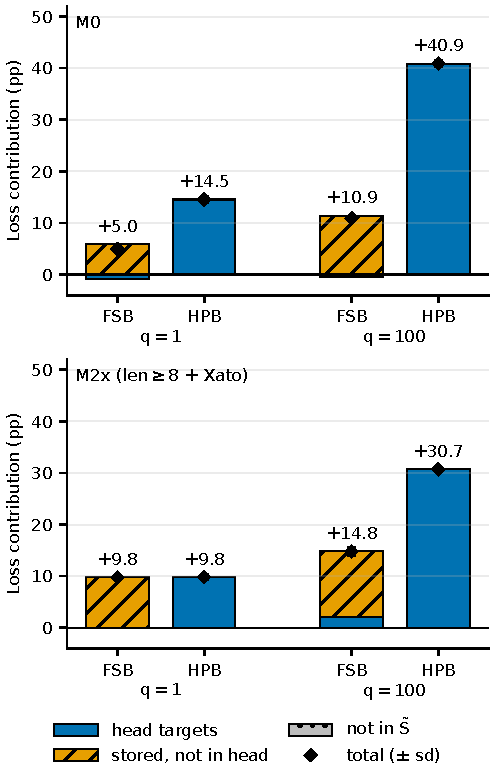
\includegraphics[width=\columnwidth]{../figs/fig3.pdf}
\caption{Which targets the emp attacker gains on (M0, $q=1$ and $q=100$; FSB $\qbar=100$ and HPB $l=12$): loss contribution = share of targets in the group $\times$ (success $-$ baseline) within the group; the three groups add up to the loss (diamond). On M0 at $q=100$ the stored-not-in-head group contributes $+11.44$ pp of the FSB total 10.92 (head $-0.51$); under HPB the head contributes all of 40.90.}
\label{fig:groups}
\end{figure}

Our explanation: FSB flattens the posterior over the passwords it believes are popular, since $\phat(w)/\gamma(w)$ is roughly the same for all of them. A rare password that was nevertheless stored has $\gamma=1$ and a count of at least 1, so its posterior in its bucket exceeds that of any head password, while the server's tail estimate puts it far below that level and est inherits the mistake. Three measurements are consistent with this: a larger head shrinks the loss (24.5, 17.5, 10.9, 7.2 and 2.3 pp for $t=100$k, 300k, 1M, 3M and 10M, at about 77 MB of client data for the 10M head against 7.5 MB for 1M); Kneser--Ney~\cite{kneser1995} and add-$\delta$ smoothing give the same loss at equal bucket size (10.14 pp on M0 at $q=100$ and 6,500 entries); and tail-only noise leaves emp at 10.88, 10.84 and 10.94 pp against 10.92 pp clean.

\subsection{A floor on $\gamma$}\label{sec:floor}

If rare stored passwords cause the loss, giving them more copies should remove it. We store every string in at least $g$ buckets (Eq.~\eqref{eq:floor}), which a client computes from its password alone. We swept $g$ from 2 to 16,384 for $\qbar\in\{10,100,1000\}$ on a development pool and ran the whole grid once on a fresh pool (both are halves of \Atest); all numbers below are from the fresh pool, where plain FSB with $\qbar=100$ loses 10.68 pp on M0. The selection rule we fixed in advance scored loss at $q=100$ against emp alone and picked $\qbar=10$ with $g=256$, beyond that configuration's own $\qbar$, so we report the grid (Table~\ref{tab:floor}). Because emp takes a count-1 password at face value, we add two attackers that hold all of $\Stilde$: gt uses $a(c)=r^*$ for a leak count $r\le 5$ and the raw count above, with the Good--Turing value
\begin{equation}\label{eq:gt}
r^*=(r+1)\,n_{r+1}/n_r,
\end{equation}
where $n_r$ is the number of stored passwords with count $r$, and est ranks by the server's estimate. We report the largest loss over the three.

\begin{table}[t]
\centering
\caption{Worst-case loss over the emp, gt and est attackers at $q=\bar q$ (fresh pool): plain FSB and FSB with a floor $g$; sizes in parentheses are relative to plain FSB.}
\label{tab:floor}
\footnotesize
\setlength{\tabcolsep}{3pt}
\begin{tabular}{llrrr}
\toprule
$\bar q$ & Scheme & Avg.\ bucket & M0 (pp) & M2x (pp) \\
\midrule
10 & plain FSB & 790 & $10.40$ & $13.44$ \\
 & floor 256 & 967 ($1.22\times$) & $0.65$ & $2.80$ \\
 & floor 1,024 & 1,516 ($1.92\times$) & $0.09$ & $1.09$ \\
\midrule
100 & plain FSB & 2,565 & $10.68$ & $14.54$ \\
 & floor 256 & 2,734 ($1.07\times$) & $3.74$ & $7.71$ \\
 & floor 1,024 & 3,276 ($1.28\times$) & $1.80$ & $4.02$ \\
 & floor 2,048 & 4,007 ($1.56\times$) & $0.08$ & $2.16$ \\
 & floor 4,096 & 5,476 ($2.14\times$) & $0.04$ & $2.16$ \\
\midrule
1000 & plain FSB & 11,336 & $10.70$ & $16.06$ \\
 & floor 2,048 & 12,722 ($1.12\times$) & $2.72$ & $6.91$ \\
 & floor 4,096 & 14,167 ($1.25\times$) & $2.19$ & $5.81$ \\
\bottomrule
\end{tabular}

\end{table}

For $\qbar=100$ a floor of 2,048 raises the average bucket from 2,565 to 4,007 entries (1.56 times) and cuts the loss from 10.68 to 0.08 pp on M0 and from 14.54 to 2.16 pp on M2x. What remains on M2x is the est attacker's policy loss, which plain FSB shows as well (2.12 pp): the floor removes the tail contribution, not the policy mismatch. At $\qbar=1000$ the floor is cheaper (1.12 times at $g=2{,}048$) but not enough (2.72 pp on M0). Unlike a larger head, it needs no client data beyond the constant $g$. It does nothing beyond $\qbar$: at $\qbar=100$ and $q=1000$ the worst case is 13.94 pp with $g=2{,}048$, while emp alone reads 0.24 pp there because it ranks count-1 passwords above the head, so a low emp loss outside $q\le\qbar$ is not evidence of safety.

\subsection{Stability across splits and cost}

We repeated the main comparison on three further independent account splits of RockYou (four in all), each with its own estimate and attackers; the floor $g=2{,}048$ was chosen on the first split's development pool, so the other three are out of sample for it. For $\qbar=100$ the worst-case loss at $q=\qbar$ on M0 is $10.96\pm0.06$ pp for plain FSB (10.89 to 11.02), $0.10\pm0.03$ pp with the floor and $41.19\pm0.20$ pp for size-matched HPB; on M2x it is $15.02\pm0.22$, $2.23\pm0.06$ and $30.68\pm0.07$ pp. The standard deviation over splits is at most 0.22 pp in every cell we measured.

A cold run of emp over all 13,125,513 stored passwords takes 14.1 s and 3.57 GB, so the attack fits on a laptop.

\section{Discussion and Limitations}

FSB's guarantee holds relative to the server's estimate and, against that attacker, with room for error. It does not hold against an attacker who holds the leak counts, who still loses to FSB more than to HPB (72 to 73\% less loss on M0). The loss sits on rare stored passwords that the estimate underrates, and a floor on $\gamma$ removes most of it for $q\le\qbar$, at 1.56 times the average bucket for $\qbar=100$.

Limitations. The leak is one corpus (RockYou), about 3\% of the 436 million passwords simulated by Li et al., and re-splitting it changes the results little but a second leak was not tested. emp, gt and est only guess stored passwords, so all numbers are lower bounds on a stronger attacker. emp uses the leak counts, which Li et al.\ already grant the attacker, but an outside observer of bucket identifiers may not have them. We model password-only checking, estimator error as independent lognormal noise, and the mechanism is supported by one intervention that does not prove it. The selection rule for the floor was a poor one, gt and est were added after the emp development run showed negative, non-monotone losses (before any fresh-pool run of them), and the floor was not run on M1b, M3 or at the scale of Li et al.; its server-side storage and lookup cost was not measured. The guarantee covers $q\le\qbar$ only, and the policy loss of 2.16 pp remains.

\section{Related Work}

HIBP sends the first five characters of a SHA-1 hash and returns the matching bucket~\cite{hunt}; Google's Password Checkup checks username-password pairs and covers over 4 billion credentials~\cite{thomas2019}. Li et al.~\cite{li2019} gave the first formal treatment of C3 services, showed that a hash prefix can raise remote guessing efficacy by a factor of 12 in some settings, and proposed FSB; they simulate on a leak of about 436 million passwords and report one policy experiment in which the estimate ignores the policy. Pal et al.~\cite{pal2022} proposed a second-generation service, and Pasquini et al.~\cite{pasquini2024} analyse its leakage to a client; we study leakage to the server and the robustness of the first-generation password-only fix. We are not aware of an earlier study that sweeps the estimation error of FSB or measures an attacker that ranks guesses by leak counts; our search was not exhaustive.

\section{Conclusion}

FSB does what it promises against the attacker it was designed for: zero loss for $q\le\qbar$, with a head estimate that can be about twice as noisy as ours. Against an attacker who holds the leak counts it leaves 10.5 to 10.9 pp of loss at $q=\qbar$ and, under a password policy, offers almost no protection at $q=1$ for $\qbar=100$. The loss comes from rare stored passwords, and a floor on $\gamma$ removes most of it for $q\le\qbar$ (0.08 pp at $\qbar=100$, 2.16 pp under the policy) without extra client data, but not for $q>\qbar$. Practitioners should state FSB's guarantee relative to the estimate and size the head or the floor against an attacker with counts. These results come from simulation on one leak (stable over four splits) against attackers that only guess stored passwords, so they are lower bounds on the leakage. Future work should test the floor at the scale of Li et al.\ and against stronger attackers, repeat the study on a second corpus used as the leak, and give the attacker generated guesses.

\textbf{Ethics.} We use public leaked-password corpora (RockYou and phpbb, via SecLists~\cite{miessler}) and simulate the server and attacker on held-out accounts; no service was contacted and no real account or live query was involved. The attacker needs only the leak and a laptop, which is why we report its cost.

\textbf{Use of generative AI.} Generative AI tools were used to help write the code and drafts of this paper. The authors reviewed the code and results and take responsibility for the content; all numbers are generated from the result files by scripts in the repository.

\textbf{Availability.} \ifblind Code, result files and the scripts that regenerate every table and number are available at a link withheld for double-blind review.\else Code, result files and the scripts that regenerate every table and number are at \url{github.com/dilpreet579/fsb-robustness-isp-paper}.\fi

\bibliographystyle{IEEEtran}
\bibliography{../refs}

\end{document}
